\documentclass[aps,prb,superscriptaddress,nofootinbib]{revtex4}
\usepackage{amsfonts}
\usepackage{amsmath}
\usepackage{amssymb}
\usepackage{graphbox}
\usepackage{graphicx}
\usepackage{caption}
\usepackage{bm}
\usepackage{bbm}
\usepackage{cancel}
\usepackage{color}
\usepackage{mathrsfs}
\usepackage[colorlinks,bookmarks=true,citecolor=blue,linkcolor=red,urlcolor=blue]{hyperref}
\usepackage{simpler-wick}
\usepackage{appendix}
\usepackage{float}
\usepackage{array}
\usepackage{booktabs}
\usepackage[export]{adjustbox}
\setlength{\parindent}{10 pt}
\setlength{\parskip}{2 pt}
\setcounter{MaxMatrixCols}{30}
\bibliographystyle{apsrev}
\newcommand{\RNum}[1]{\uppercase\expandafter{\romannumeral #1\relax}}
\newcommand{\normord}[1]{{:\mathrel{#1}:}}
\def\tbs{\textbackslash}
\def \tr{\operatorname{tr}}
\def \Tr{\operatorname{Tr}}


\begin{document}
\title{Anomaly}
\author{Jie Ren}



\maketitle

\tableofcontents



\section{Symmetries}

A (classical) symmetry means that the equation of motion dictated by a Lagrangian is invariant under the (usually infinitesimal) transformation (denoted as $\Lambda$, but not necessarily the Lorentz transformation), the coordinate and the field transform as
\begin{equation}
\begin{aligned}
	x^\mu\rightarrow {x'}^\mu = x^\mu + \omega_a \frac{\delta x^\mu}{\delta \omega_a}, \quad
	\phi(x) \rightarrow \phi'(x') = \phi(x) + \omega_a \frac{\delta \mathcal F}{\delta \omega_a}(x).
\end{aligned}
\end{equation}
Here the field $\phi$ may contain additional internal degrees of freedom. 
Also here we adopt the active view of the field transformation, meaning that for a fixed coordinate $x$, the transformation of the field is
\begin{equation}
	\delta_\omega \phi(x) \equiv \phi'(x) - \phi(x) = - i\omega_a \hat G_a \phi(x),
\end{equation}
where by comparing the definitions, we know
\begin{equation}
	\hat G_a\phi(x) = \frac{\delta x^\mu}{\delta\omega_a} \partial_\mu \phi(x) - \frac{\delta\mathcal F}{\delta\omega_a}.
\end{equation}

\subsection{Noether's Theorem}
The action under the above transformation becomes
\begin{equation}
	S' = \int d^d x' \mathcal L\left(\phi'(x'),\frac{\partial \phi'}{\partial {x'}^\mu}(x')\right).
\end{equation}
We are going to expand the expression to the first order of $\omega_a$'s.
Note that there are two contributions to the change of action: one from the coordinate change and the other from the Lagrangian.
For the coordinate part, we have
\begin{equation}
	\frac{\partial {x'}^\mu}{\partial x^\nu}
	= \delta^\mu_\nu + \partial_\nu\left(\omega_a \frac{\delta x^\mu}{\delta \omega_a}\right).
\end{equation}
Using the relation $\det(1+E) = 1 + \Tr E$ for small $E$, we know by changing the variable $x' \rightarrow x$, we get a contribution
\begin{equation}
	\delta S 
	= \int d^d x \left|\det \frac{\partial {x'}^\mu}{\partial x^\nu}\right|\left(\mathcal L + \omega_a \frac{\delta x^\mu}{\delta \omega_a} \partial_\mu \mathcal L \right)  
	= \int d^d x \ \partial_\mu \left(\mathcal L \omega_a \frac{\delta x^\mu}{\delta \omega_a}\right).
\end{equation}
On the other hand, the change of Lagrangian is
\begin{equation}
	{\delta} \mathcal L =
	\left[\frac{\partial \mathcal L}{\partial \phi} -\partial_\mu \frac{\partial\mathcal L}{\partial(\partial_\mu\phi)} \right]\delta_\omega \phi + \partial_\mu \left(\frac{\partial\mathcal L}{\partial(\partial_\mu\phi)} \delta_\omega \phi \right).
\end{equation}
The first term vanishes as the result of classical EOM.
Together, the change of action is
\begin{equation}
\begin{aligned}
	\delta S 
	&= \int d^d x \ \partial_\mu \left(\mathcal L \omega_a \frac{\delta x^\mu}{\delta \omega_a}+\frac{\partial\mathcal L}{\partial(\partial_\mu\phi)} \delta_\omega \phi \right) \\
	&= \int d^d x \ \partial_\mu \left[\left(\delta^\mu_\nu \mathcal L - \frac{\partial\mathcal L}{\partial(\partial_\mu\phi)}\partial_\nu \phi(x) \right)\frac{\delta x^\nu}{\delta\omega_a}  + \frac{\partial\mathcal L}{\partial(\partial_\mu\phi)}\frac{\delta\mathcal F}{\delta\omega_a}\right] \omega_a \\
	&\equiv \int d^d x \ \omega_a  \partial_\mu J^\mu_a.
\end{aligned} 
\end{equation}
The symmetry requires that the action is invariant over arbitrary spacetime region, so that $J_a^\mu$ is conserved current.
Note that we can freely add a derivative of an anti-symmetric tensor to the current:
\begin{equation}
	J^\mu_a \rightarrow J^\mu_a + \partial_\nu B^{\nu\mu}_a,\quad
	B^{\mu\nu} = -B^{\nu\mu}.
\end{equation}
The above discussion gives the Noether's theorem, which says that symmetries in classical field theory imply conserved quantities.

\subsection{Ward Identity}
The quantum version of the Noether's theorem is the Ward identity.
From the above discussion, we consider a \textit{local} transformation, i.e., $\omega_a(x)$ now depend on coordinate $x$.
The action under such transformation becomes:
\begin{equation}
\begin{aligned}
	S &\rightarrow \int d^d x \left[\mathcal L(x) + \partial_\mu\left( \omega_a(x) J_a^\mu \right) + \omega_a(x) F_a(x)\right] \\
	&= \int d^d x \left[\mathcal L(x) + \omega_a(x) \partial_\mu J_a^\mu + \omega_a(x) (F_a+\partial_\mu J^\mu)\right],
\end{aligned}
\end{equation}
where $\omega_a(x) F_a(x)$ comes from the classical EOM term that no longer vanishes automatically.
However, using the fact that when $\omega_a(x)$ is constant, the action is invariant (over arbitrary region), any term involving $\omega(x)$ should be zero. 
We thus know the action only depend on the derivative of $\omega_a(x)$, i.e.,
\begin{equation}
	S \rightarrow \int d^d x \left[\mathcal L(x) + J_a^\mu \partial_\mu \omega_a(x)  \right],
\end{equation}
Consider the quantum partition function $Z = \int D[\phi] e^{iS[\phi]}$.
After the infinitesimal transformation, the partition function becomes
\begin{equation}
	Z = \int D[\phi'] e^{iS[\phi]} \exp\left[-i\int d^d x \ \omega_a(x) \partial_\mu J_a^\mu (x)\right].
\end{equation}
Note that the infinitesimal transformation for path-integral is nothing but a change of variable.
If we assume the transformation does not change the measure: $D[\phi'] = D[\phi]$, then the quantum partition function is invariant under the local transformation.
This implies the operator identity:
\begin{equation}
	\partial_\mu J_a^\mu(x) = 0.
\end{equation}
Note that the operator identity should be understood as a set of identity for correlation function.
Consider the generating functional $Z[K] =\int D[\phi] \exp(iS[\phi]+ i \int d^d x K \phi)$, where we denote the auxiliary current as $K$ to avoid confusion with conserved current.
For arbitrary infinitesimal (local) symmetry transformation, the generating functional
\begin{equation}
	Z[K] = \int D[\phi] e^{iS[\phi]+ i \int d^d x K \phi} \left[1-i\int d^d x\ \omega_a(x)\left(\partial_\mu J^\mu + K \hat G \phi \right) \right]
\end{equation}
remains the same, which means
\begin{equation}
	\int D[\phi] e^{iS[\phi]+ i \int d^d x K \phi} \left(\partial_\mu J^\mu(x) + K(x) \hat G \phi(x) \right) = 0.
\end{equation}
By taking derivative on $K(x_i)$ for $n$ times, and then set $K=0$, we get the Ward identity:
\begin{equation}
	\partial_\mu \langle J_a^\mu(x) \phi(x_1) \cdots \phi(x_n)\rangle = -i\delta(x-x_i) \sum_{i=1}^n \langle \phi_1 \cdots \hat G\phi(x_i)\cdots \phi_n\rangle.
\end{equation}
The right-hand side can be viewed as the contact due to the time-ordering;
It vanishes if $x \ne x_i$ for all $i$'s. 


\section{Axial Anomaly}
In this section, we consider the axial anomaly apearing in the $(1+1)$D fermion field theory.
Note that the gamma matrices in this dimension are
\begin{equation}
	\gamma^0 = \begin{bmatrix}
		0 & -i \\ i & 0
	\end{bmatrix} ,\quad
	\gamma^1 = \begin{bmatrix}
		0 & i \\ i & 0
	\end{bmatrix},\quad
	\gamma^3 = \gamma^0 \gamma^1 = \begin{bmatrix}
		1 & 0 \\ 0 & -1
	\end{bmatrix}.
\end{equation}
Consider a massless fermion field described by the Lagrangian 
\begin{equation}
\begin{aligned}
	\mathcal L &= \bar\psi(t,x) \gamma^\mu(i\partial_\mu+eA_\mu)\psi(t,x) \\
	&= \bar\psi \begin{bmatrix}
		0 & \partial_t -ieA_t - \partial_x +ieA_x \\
		-\partial_t +ieA_t - \partial_x +ieA_x
	\end{bmatrix} \psi \\
	&= \psi^\dagger \begin{bmatrix}
		i\partial_t +eA_t +i \partial_x + eA_x \\
		0 & i\partial_t +eA_t - i\partial_x - eA_x
	\end{bmatrix} \psi,
\end{aligned}
\end{equation}
which is invariant under the axial rotation $\psi \rightarrow e^{i\theta\gamma^3}\psi$.
That is, for massless field, different chiralities are separated; we can thus define the right/left mover as
\begin{equation}
	\psi_\pm = P_\pm \psi \equiv \frac{1 \pm \gamma^3}{2}\psi.
\end{equation}
Note that the field theory has the gauge redundency
\begin{equation}
	\psi(t,x) \rightarrow e^{i\lambda(t,x)}\psi(t,x),\quad
	A_\mu(t,x) \rightarrow A_\mu(t,x)+\partial_\mu \lambda(t,x).
\end{equation}
Thus, we can choose the gauge $\lambda = -\int dt A_t$ so that $A_t=0$.
We also assume that $A_x$ is independent of $x$.
This can always be acheive by choosing a suitable gauge since thjere is no magnetic field in 1D.


\subsection{Canonical Quantization}
The canonical quantization start from the commutation relation $\{\psi_\pm(t,x),\psi^\dagger_\pm(t,y)\} = \delta(x-y)$.
The Hamiltonian density is then
\begin{equation}
	\mathcal H = \psi^\dagger \begin{bmatrix}
		-i\partial_x - eA_x & 0 \\
		0 & i\partial_x + eA_x
	\end{bmatrix} \psi.
\end{equation}
Now define the theory on a circle with radius $R$, and impose the boundary condition:
\begin{equation}
	\psi_\pm(t,0) = -\psi_\pm(t,2\pi R),\quad
	A_x(t,0) = A_x(t,2\pi R).
\end{equation}
For Dirac theory, the spectrum linearly depends on the canonical momentum, i.e., 
\begin{equation}
	E_n^{(\pm)} = \pm(p_n-A_x).
\end{equation}
The finite size system allows $p$ taking the discrete values: 
\begin{equation}
	2(2\pi R) p_n = (2n+1)2\pi \quad \Longrightarrow \quad
	p_n = \left(n-\frac{1}{2}\right)\frac{1}{R}.
\end{equation}
For notational convenience, we adopt the convention 
\begin{equation}
	E_{n_\pm} = \pm \left(n_\pm \mp \frac{1}{2} \right) \frac{1}{R} \mp A_x
\end{equation}
so that for $A_x=0$, the ground state occupies the modes $n_\pm \le 0$.
From this expression we already see the anomaly: if we adiabatically incert a unit flux such that $A_x = 1/R$, the spectrum is the same as the $A_x=0$ case, while the state will become an excited state.
We define the charge for left and right fermions:
\begin{equation}
	\hat Q_\pm \equiv \int dx \bar\psi_\pm \gamma^0 \psi_\pm.
\end{equation}
The electric charge is then $\hat Q = \hat Q_+ + \hat Q_-$, and the axial charge is $\hat Q_3 = \hat Q_+ - \hat Q_-$.
During the insertion of the unit flux, the ground state will be altered, and thus axial charge $\hat Q_3$ will change.
But since the charge is infinity in the field theory, we shall consider a suitable regularization scheme.

\subsection{Point-Splitting Regularization}
The expansion of $\psi(t,x)$ in terms of eigen modes is:
\begin{equation}
\begin{aligned}
	\psi_\pm(t,x) &= \sum_n \varphi_{\pm,n} \hat c_{\pm, n}, \\
	\varphi(t,x) &= \frac{1}{\sqrt{L}}\exp\left[\frac{i}{R}\left(n\mp \frac{1}{2}\right)(x\mp t)\pm iA_x t\right].
\end{aligned}
\end{equation}
The charge is then evaluated as
\begin{equation}
\begin{aligned}
Q_{+} &= \left\langle\Omega\left|\hat{Q}_{+}\right| \Omega\right\rangle=\sum_{n=-\infty}^0 \int_0^L d x \varphi_{+, n}^{\dagger}(x) \varphi_{+, n}(x), \\
Q_{-} &= \left\langle\Omega\left|\hat{Q}_{-}\right| \Omega\right\rangle=\sum_{n=0}^{\infty} \int_0^L d x \varphi_{-, n}^{\dagger}(x) \varphi_{-, n}(x).
\end{aligned}
\end{equation}
The summation appears to be infinite.
We use the point-splitting regulation scheme, i.e.,
\begin{equation}
	\psi_{\pm}^{\dagger}(t,x) \psi_{\pm}(t,x) \rightarrow \psi_{\pm}^{\dagger}(t,x) \exp \left(-i \int_x^{x+\varepsilon} d x^{\prime} A_x\left(x^{\prime}\right)\right) \psi_{\pm}(t,x+\varepsilon)
\end{equation}
Using the exact form of $\psi_\pm$, and the orthogonal relation, we get the regularized expression:
\begin{equation}
	Q_{+}^r=\sum_{n=0}^{\infty} \exp \left[-i\left(n+\frac{1}{2}\right) \frac{\varepsilon}{R}-i \varepsilon A_x\right], \quad Q_{-}^r=\sum_{n=0}^{\infty} \exp \left[i\left(n+\frac{1}{2}\right) \frac{\varepsilon}{R}-i \varepsilon A_x\right].
\end{equation}
The series does not converge, but we could add a small imaginary part to $\varepsilon$ to remedy this.
Formally, we have
\begin{equation}
	Q^r_+ = \frac{e^{-i\varepsilon A_x}}{e^{+i \varepsilon/2R}-e^{-i \epsilon/2R}} 
	\simeq \frac{R}{i \varepsilon}-R A_x, \quad
	Q_{-}^r=-\frac{R}{i \varepsilon}+R A_x
\end{equation}
After subtracting the infinity, we have $Q_5 = - 2R A_x$.
This leads to the expression of the axial anomaly:
\begin{equation}
	\dot Q_5 = -2R \dot A_x = -\oint \frac{dx}{\pi} E^x(x,t) = \int \frac{dx}{2\pi}\epsilon^{\mu\nu}F_{\mu\nu} = \int dx\ \partial_\mu J_3^\mu \quad \Longrightarrow \quad
	\partial_\mu J_3^\mu = \frac{\epsilon^{\mu\nu}}{2\pi} F_{\mu\nu}.
\end{equation}
If we consider an adiabatic insertion of a unit flux, by identifying $\pm T$, the amount of axial charge difference is a topological quantity, given by the \textit{first Chern class}:
\begin{equation}
	\Delta Q_5 = 2I[A], \quad
	I[A] = \int \frac{d^2 x}{4\pi} \epsilon^{\mu\nu}F_{\mu\nu} \in \mathbbm Z.
\end{equation}






\section{Chiral Anomaly}


Most of the time, a classical symmetry is also a symmetry of the quantum theory based on the same Lagrangian.
When it is not, the symmetry is said to be \textit{anomalous}.
For classical field described by the Lagrangian $\mathcal L[\phi]$, for an infinitesimal transformation 
\begin{equation}
	\delta\phi = \epsilon(x) X \phi(x),
\end{equation}
the Lagrangian transforms as
\begin{equation}
\begin{aligned}
	\delta \mathcal L 
	&= \frac{\partial \mathcal L}{\partial(\partial_\mu \phi)} \partial_\mu[\epsilon(x) X \phi(x)] + \frac{\partial \mathcal L}{\partial \phi} \epsilon(x) X \phi(x) \\
	&= \frac{\partial \mathcal L}{\partial(\partial_\mu \phi)}X \phi (\partial_\mu\epsilon) + \left[\frac{\partial \mathcal L}{\partial \phi}X\phi + \frac{\partial \mathcal L}{\partial(\partial_\mu \phi)}\partial_\mu X \phi \right]\epsilon.
\end{aligned}
\end{equation}
For a symmetry transformation, when $\epsilon(x)$ is constant, $\delta \mathcal L = 0$, we know the expression in the bracket is zero, which is just the classical equation of motion.
We can define what is left as the current:
\begin{equation}
	\delta \mathcal L = \left[\frac{\partial \mathcal L}{\partial(\partial_\mu \phi)}X \right] \partial_\mu\epsilon(x)
	\equiv J^\mu(x) \partial_\mu \epsilon(x).
\end{equation}
The action is
\begin{equation}
	\delta S = \int d^d x \delta \mathcal L 
	= -\int d^d x\ \epsilon(x) \partial_\mu J^\mu(x),
\end{equation}
which is true for all $\epsilon(x)$ configuration, which implies $\partial_\mu J^\mu(x) = 0$.
This statement is Noether's theorem, saying that symmetries lead to conserved currents.
For quantum field theory, $J^\mu(x)$ is an operator, not a number.
To see what Noether's theorem means, consider the quantum partition functional $Z = \int D[\phi] e^{iS[\phi]}$.
After the infinitesimal axial transformation, the partition function becomes
\begin{equation}\label{eq:AN-partition-1}
	Z = \int D[\phi'] e^{iS[\phi]} \exp\left[-i\int d^d x \ \epsilon(x) \partial_\mu J^\mu (x)\right].
\end{equation}
Since the change of variable will have no effect on the functional integral, the partition function (\ref{eq:AN-partition-1}) will not change under the transformation.
If we assume the transformation does not change the measure, i.e.,
\begin{equation}\label{eq:AN-measure-eq}
	D[\phi'] = D[\phi],
\end{equation}
then, since Eq.~(\ref{eq:AN-partition-1}) stands for any $\epsilon(x)$, we must have the operator identity: $\partial_\mu J^\mu(x) = 0$.
For the case of anomalies, however, Eq.~(\ref{eq:AN-measure-eq}) is no longer true.
The change of measure will break the classical symmetries.

For the massless Dirac field Lagrangian $\mathcal L = i\bar\psi \cancel D \psi$, the chiral (axial) rotation 
\begin{equation}
	\psi \rightarrow e^{i\epsilon \gamma^5}\psi, \quad
	\bar\psi \rightarrow \bar\psi e^{i\epsilon \gamma^5}
\end{equation}
is a classical symmetry of the action.
Noether's theorem gives the conserved current
\begin{equation}
	J^\mu_5 = \frac{\partial \mathcal L}{\partial(\partial_\mu \psi)} i\gamma^5\psi = \bar\psi \gamma^\mu \gamma^5\psi.
\end{equation}
After the infinitesimal axial transformation, the quantum partition function becomes:
\begin{equation}\label{eq:AN-CH-partition}
\begin{aligned}
	Z &= \int D[\bar\psi,\psi] \exp\left[i\int d^d x\ \bar\psi(x) e^{i\epsilon(x)\gamma^5}\gamma^\mu(i\partial_\mu - e A_\mu) e^{i\epsilon(x)\gamma^5}\psi(x) \right] \\
	&= \int D[\bar\psi',\psi'] \exp\left\{i\int d^d x\ \bar\psi(x) \gamma^\mu\left[iD_\mu-\partial_\mu\epsilon(x)\gamma^5\right] \psi(x) \right\} \\
	&= \int D[\bar\psi,\psi] e^{iS[\bar\psi,\psi]} \mathcal J^2 \exp\left[i \int d^d x\ \epsilon(x) \partial_\mu J_5^\mu(x) \right],
\end{aligned}
\end{equation}
where $\mathcal J$ is the Jacobian:
\begin{equation}
	\mathcal J = \det\left(\frac{D[\bar\psi']}{D[\bar\psi]}\right)^{-1}=\det\left(\frac{D[\psi']}{D[\psi]}\right)^{-1}.
\end{equation}
Note that in contrast to the c-number calculus, since the integration of a Grassmann variable is algebraically identical to differentiation, the Jacobian for the change of variable is the inverse of the determinant.


\subsection{Anomaly in the Measure}

We now going to evaluate the Jacobian for the measure:
\begin{equation}
	\mathcal J = \exp\left(-i \int d^d x \ \epsilon(x) \Tr[\gamma^5] \right),
\end{equation}
where $\mathcal A = \Tr[\gamma^5]$.
Note that the trace is over all eigenstates of the Hamiltonian (Lagrangian).
The orthonormal basis for the (massless) Dirac equation is:
\begin{equation}
	\gamma^\mu (\partial_\mu + ie A_\mu ) \xi_k(x) = E_k \xi_k(x), \quad
	\bar\eta_k(x) \left(\overleftarrow\partial_\mu -ieA_\mu\right) \gamma^\mu = E_k \bar\eta_k(x).
\end{equation}
Note that the subscript $k$ is the label for the eigenstate (or wave function).
It is to be differentiated from the state in the momentum space.
The trace is carried out as
\begin{equation}\label{eq:AN-tr-1}
	\Tr\left[\gamma^5\right] 
	= \int \frac{d^d k}{(2\pi)^d} \tr\left[\bar\eta_k \gamma^5 \xi_k \right],
\end{equation}
where we distinguish the small $\tr$ as the trace over the spinor indices. 
The integral (\ref{eq:AN-tr-1}) is divergent, the simplest regulation would be putting a heat-kernel regulator to the expression, i.e., by putting a gaussian regulator suppressing the large momenta:
\begin{equation}
	\exp\left(\frac{\cancel{\Pi}^2}{\Lambda^2}\right)
	= \exp\left[\frac{(\cancel{k}-e\cancel{A})^2}{\Lambda^2}\right].
\end{equation}
Such a Gaussian regulator, when the functional integral is converted to Euclidean space, provides a Gaussian suppression for large momenta.
Here, to preserve the gauge invariance, the canonical momentum $\Pi$ as the eigenvalue of the covariant derivative should be used instead of mechanical momentum. 
Note that
\begin{equation}
\begin{aligned}
	(\cancel D)^2 &= \gamma^\mu \gamma^\nu {D}_\mu {D}_\nu 
	= \frac{1}{2} \{\gamma^\mu,\gamma^\nu\} {D}_\mu {D}_\nu + [\gamma^\mu,\gamma^\nu] {D}_\mu {D}_\nu \\
	&= \left(\partial_\mu+ie A_\mu \right)^2 + \frac{1}{2} \gamma^\mu \gamma^\nu \left[\partial_\mu+ie A_\mu, \partial_\nu+ie A_\nu \right] \\
	&= \left(\partial_\mu+ie A_\mu \right)^2 + \frac{ie}{2}\gamma^\mu \gamma^\nu F_{\mu\nu},
\end{aligned}
\end{equation}
which implies
\begin{equation}
	\cancel{\Pi}^2 = \Pi^2 - \frac{ie}{2}\gamma^\mu \gamma^\nu F_{\mu\nu}.
\end{equation}
The trace of $\gamma^5$ with the Gaussian regulator is
\begin{equation}
	\Tr\left[\gamma^5\right] 
	= \int \frac{d^d k}{(2\pi)^d} \tr\left[\bar\eta_k \gamma^5 e^{\cancel{\Pi}^2/\Lambda^2}\xi_k \right] 
	= \int \frac{d^d k}{(2\pi)^d} e^{(k-eA)^2/\Lambda^2}\tr\left[\gamma^5 \exp\left(-\frac{ie}{2\Lambda^2} \gamma^\mu \gamma^\nu F_{\mu\nu}\right)\right].
\end{equation}
Shift $k \rightarrow k + e A$, and then expand the exponential according to the order of $\Lambda^{-1}$:
\begin{equation}
\begin{aligned}
	\exp\left(-\frac{ie}{2\Lambda^2} \gamma^\mu \gamma^\nu F_{\mu\nu}\right)
	=&\ 1-\frac{ie}{2\Lambda^2} \gamma^\mu \gamma^\nu F_{\mu\nu}-\frac{e^2}{8\Lambda^4} \gamma^\mu \gamma^\nu \gamma^\rho \gamma^\sigma F_{\mu\nu} F_{\rho\sigma} + O\left(\frac{1}{\Lambda^6}\right).
\end{aligned}
\end{equation}
For $d=4$ case, the only term surviving the gamma trace is
\begin{equation}
	\mathrm{tr} \left[\gamma^5 \gamma^\mu \gamma^\nu \gamma^\rho \gamma^\sigma \right] 
	= -4i\varepsilon^{\mu\nu\rho\sigma}.
\end{equation}
The trace formula (\ref{eq:AN-tr-1}) is then
\begin{equation}
	\Tr[\gamma^5] = \lim_{\Lambda\rightarrow\infty} \frac{ie^2}{2\Lambda^4} \int \frac{d^4k}{(2\pi)^4} e^{\frac{k^2}{\Lambda^2}}  \varepsilon^{\mu\nu\rho\sigma}F_{\mu\nu} F_{\rho\sigma}.
\end{equation}
Now we do the Wick rotation $k^0 \rightarrow -k^0$. 
The trace then becomes
\begin{equation}
	\Tr[\gamma^5] = \lim_{\Lambda\rightarrow\infty} \frac{-e^2}{2\Lambda^4} \int \frac{\Omega_4 k^3_E dk_E}{(2\pi)^4} e^{-\frac{k_E^2}{\Lambda^2}}  \varepsilon^{\mu\nu\rho\sigma}F_{\mu\nu} F_{\rho\sigma} 
	= -\frac{e^2}{32\pi^2} \varepsilon^{\mu\nu\rho\sigma}F_{\mu\nu} F_{\rho\sigma}.
\end{equation}
Now return to Eq.~(\ref{eq:AN-CH-partition}), the final result is
\begin{equation}
	Z = \int D[\bar\psi,\psi] e^{iS[\bar\psi,\psi]} \exp\left[i\int d^d x \ \epsilon(x) \left(\partial_\mu J_5^\mu+ \frac{e^2}{16\pi^2}\varepsilon^{\mu\nu\rho\sigma}F_{\mu\nu} F_{\rho\sigma}\right)\right].
\end{equation}
We thus have
\begin{equation}
	\partial_\mu J^\mu_5 = -\frac{e^2}{16\pi^2}\varepsilon^{\mu\nu\rho\sigma}F_{\mu\nu} F_{\rho\sigma}.
\end{equation}

If we instead consider the quantum field theory on 2d spacetime, the trace of gamma matrices satisfies:
\begin{equation}
	\tr[\gamma^5 \gamma^\mu \gamma^\nu] = 2 \varepsilon^{\mu\nu}.
\end{equation}
The trace formula then becomes
\begin{equation}
\begin{aligned}
	\Tr[\gamma^5] 
	&= i\int \frac{d^2 k_E}{(2\pi)^2} e^{-k_E^2/\Lambda^2}\tr\left[\gamma^5 \exp\left(-\frac{ie}{2\Lambda^2} \gamma^\mu \gamma^\nu F_{\mu\nu}\right)\right] \\
	&= \frac{e}{2\Lambda^2} \int \frac{d^2 k_E}{(2\pi)^2} e^{-k_E^2/\Lambda^2}\tr\left[\gamma^5 \gamma^\mu \gamma^\nu \right]F_{\mu\nu} \\
	&= \frac{e}{4\pi}\varepsilon^{\mu\nu}F_{\mu\nu}.
\end{aligned}
\end{equation}
We thus have
\begin{equation}
	\partial_\mu J^\mu_5 = \frac{e}{2\pi} \varepsilon^{\mu\nu} F_{\mu\nu}.
\end{equation}
In general, for $d=2n$ case, 
\begin{equation}
	\tr[\gamma^5 \gamma^{\mu_1}\cdots \gamma^{\mu_{2n}}] = (-i)^{n-1} 2^n \varepsilon^{\gamma^{\mu_1}\cdots \gamma^{\mu_{2n}}}
\end{equation}
The crucial part of the calculation is
\begin{equation}
\begin{aligned}
	\tr\left[\gamma^5 \exp\left(-\frac{ie}{2\Lambda^2} \gamma^\mu \gamma^\nu F_{\mu\nu}\right)\right] 
	&=\frac{1}{n!}\left(-\frac{ie}{2\Lambda^2}\right)^n \tr[\gamma^5 \gamma^{\mu_1}\cdots \gamma^{\mu_{2n}}] F_{\mu_1\mu_2}\cdots F_{\mu_{2n-1}\mu_{2n}} \\
	&=(-1)^n i \frac{e^n}{n! \Lambda^{2n}} \varepsilon^{\gamma^{\mu_1}\cdots \gamma^{\mu_{2n}}} F_{\mu_1\mu_2}\cdots F_{\mu_{2n-1}\mu_{2n}}
\end{aligned}
\end{equation}
The trace is then
\begin{equation}
\begin{aligned}
	\Tr[\gamma^5] 
	&= (-1)^{n+1} \frac{e^n}{n! \Lambda^{2n}}\varepsilon^{\gamma^{\mu_1}\cdots \gamma^{\mu_{2n}}} F_{\mu_1\mu_2}\cdots F_{\mu_{2n-1}\mu_{2n}} \int \frac{d^d k_E}{(2\pi)^d} e^{-k_E^2/\Lambda^2} \\
	&= (-1)^{n+1} \frac{e^n}{n! (4\pi)^n} \varepsilon^{\gamma^{\mu_1}\cdots \gamma^{\mu_{2n}}} F_{\mu_1\mu_2}\cdots F_{\mu_{2n-1}\mu_{2n}}.
\end{aligned}
\end{equation}
which leads to
\begin{equation}
	\partial_\mu J^\mu_5 = (-1)^{n+1} \frac{2 e^n}{n! (4\pi)^n} \varepsilon^{\gamma^{\mu_1}\cdots \gamma^{\mu_{2n}}} F_{\mu_1\mu_2}\cdots F_{\mu_{2n-1}\mu_{2n}}.
\end{equation}






\subsection{Triangle Diagram}
The trace (\ref{eq:AN-tr-1}) can be rewritten as $\Tr[\gamma^5] = -\mathrm{tr}[\gamma^5 iG_F(x,x)]$.
The Fermion propagator in the presence of the background field is
\begin{equation}
\begin{aligned}
	iG_F(x_1,x_2) =&\ iG^0_F(x_1,x_2) + iG^0_F(x_1,y)[-ie\cancel{A}(y)]iG^0_F(y,x_2) \\
	& + iG^0_F(x_1,y_1)[-ie\cancel{A}(y_1)]iG^0_F(y_1,y_2)[-ie\cancel{A}(y_2)]iG^0_F(y_2,x_2).
\end{aligned}
\end{equation}
From previous discussion, it suggests that the chiral anomaly appears in the second order perturbation theory.
We thus consider the second order one-loop diagram (sometimes known as the triangle diagram):
\begin{equation}
\begin{aligned}
	i\mathcal{M}^{\mu\nu\rho}(p_1,p_2,q)
	=&\ 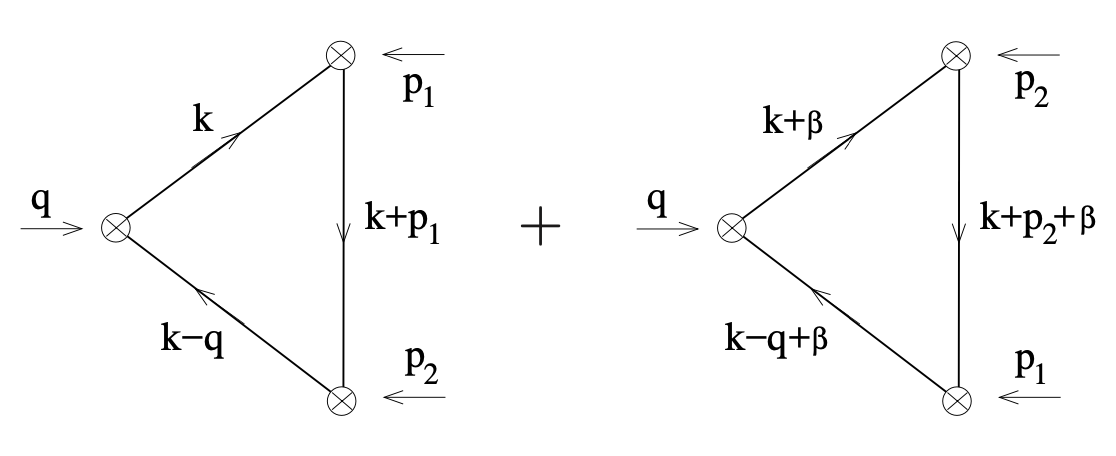
\includegraphics[width=0.4\linewidth,align=c]{pics/AN-Tri.png} \\
	=&\ -\int \frac{d^{4} k}{(2 \pi)^{4}} \tr\left[\frac{i}{\cancel k} \gamma^{\rho} \gamma^{5} \frac{i}{\cancel k-\cancel q} \gamma^{\nu} \frac{i}{\cancel k+\cancel p_{1}} \gamma^{\mu} \right]  \\
	&\ -\int \frac{d^{4} k}{(2 \pi)^{4}} \tr\left[\frac{i}{\cancel k + \cancel \beta} \gamma^{\rho} \gamma^{5} \frac{i}{\cancel k-\cancel q +\cancel \beta} \gamma^{\mu} \frac{i}{\cancel k+\cancel p_{2}+\cancel \beta} \gamma^{\nu}\right]
\end{aligned}
\end{equation}
To the derivative of the axial current is related to the amplitude
\begin{equation}
\begin{aligned}
	q_\rho \mathcal{M}^{\mu\nu\rho} 
	=&\ \int \frac{d^{4} k}{(2 \pi)^{4}} \tr\left[\frac{1}{\cancel k} (\cancel{q}-\cancel{k}+\cancel{k}) \gamma^{5} \frac{1}{\cancel k-\cancel q} \gamma^{\nu} \frac{1}{\cancel k+\cancel p_{1}} \gamma^\mu \right] + \\
	&\ \int \frac{d^{4} k}{(2 \pi)^{4}} \tr\left[\frac{1}{\cancel k +\cancel \beta} (\cancel{q}-\cancel{k}-\cancel \beta +\cancel{k} +\cancel\beta) \gamma^{5} \frac{1}{\cancel k-\cancel q+\cancel\beta} \gamma^{\mu} \frac{1}{\cancel k+\cancel p_{2}+\cancel \beta} \gamma^\nu \right] \\
	=&\ \int \frac{d^{4} k}{(2 \pi)^{4}} \tr\left[\gamma^{5} \frac{1}{\cancel k+\cancel p_{1}} \gamma^\mu \frac{1}{\cancel k-\cancel q} \gamma^{\nu}  -  \gamma^{5}   \frac{1}{\cancel k+\cancel p_{1}} \gamma^\mu \frac{1}{\cancel k} \gamma^{\nu} \right]+ \\
	&\ \int \frac{d^{4} k}{(2 \pi)^{4}} \tr\left[\gamma^{5} \frac{1}{\cancel k-\cancel q+\cancel\beta} \gamma^{\mu} \frac{1}{\cancel k+\cancel p_{2}+\cancel \beta} \gamma^\nu -\gamma^5\frac{1}{\cancel k+\cancel\beta}\gamma^\mu\frac{1}{\cancel k+\cancel p_2+\cancel\beta}\gamma^\nu\right] \\
	\equiv &\ \Delta^{\mu\nu}_1 + \Delta^{\mu\nu}_2,
\end{aligned}
\end{equation}
where we define
\begin{equation}\label{eq:AN-Tri-div-int}
\begin{aligned}
	\Delta^{\mu\nu}_1 &= \int \frac{d^{4} k}{(2 \pi)^{4}} \tr\left[
		\gamma^{5} \frac{1}{\cancel k+\cancel p_{1}} \gamma^\mu \frac{1}{\cancel k+\cancel p_1+\cancel p_2} \gamma^{\nu} -
		\gamma^5\frac{1}{\cancel k+\cancel\beta}\gamma^\mu\frac{1}{\cancel k+\cancel p_2+\cancel\beta}\gamma^\nu 
	\right], \\
	\Delta^{\mu\nu}_2 &= \int \frac{d^{4} k}{(2 \pi)^{4}} \tr\left[
		\gamma^{5} \frac{1}{\cancel k+\cancel p_1 +\cancel p_2+\cancel\beta} \gamma^{\mu} \frac{1}{\cancel k+\cancel p_{2}+\cancel \beta} \gamma^\nu -
		\gamma^{5}   \frac{1}{\cancel k+\cancel p_{1}} \gamma^\mu \frac{1}{\cancel k} \gamma^{\nu}
	\right].
\end{aligned}
\end{equation}
We come across a similar situation where the expression, although naively appears to be zero, is actually (linearly) divergent and may produce a finite number when introducing a regulator.
However, usual regulators fail in this specific case.
The dimensional regularization is not suitable since the chiral fermions are a feature of four dimensions.
Pauli-Villars, which would introduce a heavy fermion, will not work either, since the fermion mass explicitly breaks the chiral symmetry we are trying to verify. 
Instead, we proceed by trying to make sense of the linearly divergent integrals directly.

Consider the one-dimensional integral
\begin{equation}
	\Delta(a) = \int^{+\infty}_{-\infty} dx \left[f(x+a)-f(x)\right],
\end{equation}
where the function $f(x)$ approaches to constants in both $x \rightarrow \pm\infty$ limit.
We can evaluate the integral by Taylor expansion:
\begin{equation}
	\Delta(a) = \int^{+\infty}_{-\infty} dx \left[af'(x)+\frac{a^2}{2}f''(x)+\cdots\right]
	= a\left[f(+\infty)-f(-\infty)\right],
\end{equation}
where the higher-derivative terms do not contribute since $f(\pm\infty)\rightarrow \text{const}$. 
In four dimensions, we can do a similar thing.
In this case, we are evaluating the integral
\begin{equation}
	\Delta(a) 
	= \int \frac{d^4k}{(2\pi)^4} \left[F(k+a)-F(k)\right] 
	= i\int \frac{d^4k_E}{(2\pi)^4} \left[\frac{\partial F}{\partial k_E^\rho} a^\rho + \frac{1}{2} \frac{\partial^2 F}{\partial k_E^\rho \partial k_E^\sigma} a^\rho a^\sigma + \cdots\right].
\end{equation}
If the integral of $F(k)$ is linearly divergent, only the first term contributes, and the result is just the integral over the surface:
\begin{equation}
	\Delta(a) = a^\rho \lim_{k\rightarrow \infty} \int \frac{d^3 S_\rho}{(2\pi)^4} F(k_E) 
	= a^\rho \lim_{k\rightarrow \infty} \int \frac{k^2_E k_{E\rho} d \Omega_4}{(2\pi)^4} F(k_E).
\end{equation}
To evaluate the integrals (\ref{eq:AN-Tri-div-int}), we just need to consider the function
\begin{equation}
\begin{aligned}
	\lim_{k\rightarrow \infty} F 
	&= \lim_{k\rightarrow \infty} \tr\left[\gamma^{5} \frac{1}{\cancel k + \cancel p} \gamma^\mu \frac{1}{\cancel k+\cancel q}\gamma^{\nu}\right]
	= -4i \varepsilon^{\rho\mu\sigma\nu} \lim_{k\rightarrow \infty} \frac{k_\rho q_\sigma + p_\rho k_\sigma + p_\rho q_\sigma}{(k+p)^2 k^2} \\
	&= -4i \varepsilon^{\rho\mu\sigma\nu} \frac{k_\rho q_\sigma + p_\rho k_\sigma + p_\rho q_\sigma}{k^4}.
\end{aligned}
\end{equation}
We then have
\begin{equation}\label{eq:AN-CH-int-form}
\begin{aligned}
	\Delta(a) 
	&= 4 \varepsilon^{\rho\mu\sigma\nu} a^\tau \int \frac{d \Omega_4}{(2\pi)^4} \frac{k_\tau (k_\rho q_\sigma + p_\rho k_\sigma + p_\rho q_\sigma)}{k^2} 
	= 4 \varepsilon^{\rho\mu\sigma\nu} a^\tau \frac{\Omega_4}{(2\pi)^4} \frac{\delta_{\tau\rho}q_\sigma + \delta_{\tau\sigma}p_\rho}{4} \\
	&= \frac{1}{8\pi^2} \varepsilon^{\mu\nu\rho\sigma} (p-q)_\rho a_\sigma.
\end{aligned}
\end{equation}
For $\Delta_{1}^{\mu\nu}$, $p=\beta$, $q=p_2+\beta$ and $a=p_1-\beta$, Eq.~(\ref{eq:AN-CH-int-form}) gives
\begin{equation}
	\Delta^{\mu\nu}_1 = \frac{1}{8\pi^2} \varepsilon^{\mu\nu\rho\sigma} (p_1-\beta)_\rho p_{2\sigma}.
\end{equation}
For $\Delta_2^{\mu\nu}$, $p=p_1$, $q=0$, and $a=p_2+\beta$, Eq.~(\ref{eq:AN-CH-int-form}) gives
\begin{equation}
	\Delta^{\mu\nu}_2 = \frac{1}{8\pi^2} \varepsilon^{\mu\nu\rho\sigma} p_{1\rho}(p_2+\beta)_\sigma.
\end{equation}
The sum of two terms is
\begin{equation}
	q_\rho \mathcal{M}^{\mu\nu\rho}(p_1,p_2,q) = \frac{1}{8\pi^2} \varepsilon^{\mu\nu\rho\sigma} \left[2 p_{1\rho} p_{2\sigma} + (p_1+p_2)_\rho \beta_\sigma \right].
\end{equation}

The result leaves us a free parameter $\beta$.
To see what is the best choice of $\beta$, we recall that the Ward identity requires
\begin{equation}
	p_{1\mu} \mathcal{M}^{\mu\nu\rho}(p_1,p_2,q) = 0.
\end{equation}
A self-consistent gauge symmetry should be anomalous-free, i.e., the Ward identity should always be satisfies, and to each order perturbation. 
The left hand side for a specific choice of $\beta$, for the one-loop diagram gives the result
\begin{equation}
\begin{aligned}
	p_{1\mu} \mathcal{M}^{\mu\nu\rho} 
	=&\ \int \frac{d^{4} k}{(2 \pi)^{4}} \left\{\tr\left[\frac{1}{\cancel k} \gamma^\rho \gamma^{5} \frac{1}{\cancel k-\cancel q} \gamma^{\nu} \frac{1}{\cancel k+\cancel p_{1}} (\cancel p_1 +\cancel k -\cancel k) \right] \right. + \\
	&\ \left.\tr\left[\frac{1}{\cancel k +\cancel \beta} \gamma^\rho \gamma^{5} \frac{1}{\cancel k-\cancel q+\cancel\beta} (\cancel k -\cancel q +\cancel \beta -\cancel k -\cancel p_2-\cancel \beta) \frac{1}{\cancel k+\cancel p_{2}+\cancel \beta} \gamma^\nu \right]\right\} \\
	=&\ \int \frac{d^{4} k}{(2 \pi)^{4}} \tr\left[\gamma^{5} \frac{1}{\cancel k - \cancel q} \gamma^\nu \frac{1}{\cancel k} \gamma^{\rho} - \gamma^{5} \frac{1}{\cancel k - \cancel q} \gamma^\nu \frac{1}{\cancel k+\cancel p_1} \gamma^{\rho}\right]+ \\
	&\ \int \frac{d^{4} k}{(2 \pi)^{4}} \tr\left[\gamma^{5} \frac{1}{\cancel k+\cancel p_2+\cancel\beta} \gamma^{\nu} \frac{1}{\cancel k+\cancel \beta} \gamma^\rho -\gamma^5\frac{1}{\cancel k-\cancel q+\cancel\beta}\gamma^\nu\frac{1}{\cancel k+\cancel\beta}\gamma^\rho\right] \\
	\equiv &\ \tilde\Delta^{\mu\nu}_1 + \tilde\Delta^{\mu\nu}_2,
\end{aligned}
\end{equation}
where we have defined
\begin{equation}
\begin{aligned}
	\tilde\Delta^{\mu\nu}_1 &= \int \frac{d^{4} k}{(2 \pi)^{4}} \tr\left[
		\gamma^{5} \frac{1}{\cancel k + \cancel p_1 +\cancel p_2} \gamma^\nu \frac{1}{\cancel k} \gamma^{\rho} -
		\gamma^5\frac{1}{\cancel k+ \cancel p_1 +\cancel p_2+\cancel\beta}\gamma^\mu\frac{1}{\cancel k+\cancel\beta}\gamma^\nu 
	\right], \\
	\tilde\Delta^{\mu\nu}_2 &= \int \frac{d^{4} k}{(2 \pi)^{4}} \tr\left[
		\gamma^{5} \frac{1}{\cancel k+\cancel p_2+\cancel\beta} \gamma^{\nu} \frac{1}{\cancel k+\cancel \beta} \gamma^\rho -
		\gamma^{5} \frac{1}{\cancel k + \cancel p_1+\cancel p_2} \gamma^\nu \frac{1}{\cancel k+\cancel p_1} \gamma^{\rho}
	\right].
\end{aligned}
\end{equation}
For $\tilde\Delta_{1}^{\mu\nu}$, $p=\beta+p_1+p_2$, $q=\beta$ and $a=-\beta$, Eq.~(\ref{eq:AN-CH-int-form}) gives
\begin{equation}
	\tilde\Delta^{\mu\nu}_1 = -\frac{1}{8\pi^2} \varepsilon^{\mu\nu\rho\sigma} (p_1+p_2)_\rho \beta_{\sigma}.
\end{equation}
For $\tilde\Delta_2^{\mu\nu}$, $p=p_1+p_2$, $q=p_1$, and $a=\beta-p_1$, Eq.~(\ref{eq:AN-CH-int-form}) gives
\begin{equation}
	\tilde\Delta^{\mu\nu}_2 = \frac{1}{8\pi^2} \varepsilon^{\mu\nu\rho\sigma} (p_1-\beta)_\rho p_{2\sigma}.
\end{equation}
The sum gives
\begin{equation}
	p_{1\mu} \mathcal{M}^{\mu\nu\rho}(p_1,p_2,q) = \frac{1}{8\pi^2} \varepsilon^{\mu\nu\rho\sigma} p_{1\rho}(p_{2}-\beta)_\sigma.
\end{equation}
Using the symmetry of the diagram, we can make the exchange ($p_1 \leftrightarrow p_2$, $\mu \leftrightarrow \nu$), which inverse the loop direction and thus change the sign of $\beta$.
We immediately get
\begin{equation}
	p_{2\nu} \mathcal{M}^{\mu\nu\rho}(p_1,p_2,q) = -\frac{1}{8\pi^2} \varepsilon^{\mu\nu\rho\sigma} p_{2\rho}(p_{1}+\beta)_\sigma.
\end{equation}
Note that the sum of three terms is independent of $\beta$:
\begin{equation}
	(p_{1\mu}+p_{2\nu}+q_{\rho}) \mathcal M^{\mu\nu\rho}(p_1,p_2,q) = \frac{1}{2\pi^2} \varepsilon^{\mu\nu\rho\sigma} p_{1\rho} p_{2\sigma}.
\end{equation}
To enforce Ward identity, the only choice we have is $\beta = p_2-p_1$, which lead to
\begin{equation}
	q_\rho \mathcal{M}^{\mu\nu\rho}(p_1,p_2,q) = \frac{1}{2\pi^2} \varepsilon^{\mu\nu\rho\sigma} p_{1\rho} p_{2\sigma}.
\end{equation}
We remark that in the path-integral formalism where we directly calculate the Jacobian of the measure, the heat-kernel regulator ensures the gauge invariant, so the Ward identity of the vector current is automatically ensured, at the expense of chiral symmetry.

The vertex function for the axial current and gauge field interaction is
\begin{equation}
	\Gamma_A^{\mu\nu\rho}(p_1,p_2,q) = -e^2 \mathcal{M}^{\mu\nu\rho}(p_1,p_2,q).
\end{equation}
Also, note that because of the symmetry, in the effective action, the contribution from this vertex is $\frac{1}{2}\Gamma_A^{\mu\nu\rho}$. 
The expectation of axial current derivative $\partial_\mu J_5^\mu(x)$ in the presence of back ground field $A(x)$ is then
\begin{equation}
\begin{aligned}
	\langle \partial_\mu J_5^\mu(x) \rangle 
	&= \frac{1}{2} \int \frac{d^4 q}{(2\pi)^4}\frac{d^4 p_1}{(2\pi)^4}\frac{d^4 p_2}{(2\pi)^4} e^{-i(q+p_1+p_2)x} q_\rho \Gamma^{\mu\nu\rho} \tilde A_\mu(p_1) \tilde A_\nu(p_2) \\
	&= -\frac{e^2}{4\pi^2} \int \frac{d^4 q}{(2\pi)^4}\frac{d^4 p_1}{(2\pi)^4}\frac{d^4 p_2}{(2\pi)^4} e^{-i(q+p_1+p_2)x} \varepsilon^{\mu\nu\rho\sigma} p_{1\rho} \tilde A_\mu(p_1) p_{2\sigma} \tilde A_\nu(p_2) \\
	&= -\frac{e^2}{4\pi^2} \int \frac{d^4 q}{(2\pi)^4}\frac{d^4 p_1}{(2\pi)^4}\frac{d^4 p_2}{(4\pi)^4} e^{-i(q+p_1+p_2)x} \varepsilon^{\mu\nu\rho\sigma} \left(-\frac{1}{4}\right)\tilde F_{\rho\mu}(p_1) \tilde F_{\sigma\nu}(p_2) \\
	&= -\frac{e^2}{16\pi^2} \varepsilon^{\mu\nu\rho\sigma} F_{\mu\nu}(x) F_{\rho\sigma}(x)
\end{aligned}
\end{equation}
In the above calculation, we use the Fourier transformed 
\begin{equation}
	\tilde F_{\mu\nu}(p) = \int \frac{d^4 x}{(2\pi)^4} e^{ipx} \partial_{[\mu} A_{\nu]}
	= i p_{[\mu} \tilde A_{\nu]}(p).
\end{equation}
The one-loop calculation tells us that all information of the chiral anomaly lies in the triangle diagram.
Sometimes, it is called that the chiral anomaly is one-loop exact.



\section{Gauge Anomaly}
While anomalies in global symmetry are physically interesting, anomalies in gauge symmetries render the theory mathematically inconsistent, since the gauge is not a symmetry, but a redundancy in describing the system.
If we wish to build a consistent theory, we must make sure that all gauge anomaly vanish.

\subsection{Chiral Fermions}
If the fermion field is massless, in the Dirac Lagrangian, the left- and right- handed spinors are formally decoupled.
One may wonder if we can build a QED with only left-handed massless Weyl fermions.
The answer is no, since the U(1) gauge field will be anomalous.

Now consider the triangle diagram with three QED vertices:
\begin{equation}
	i\mathcal M^{\mu\nu\rho}(p,q,r) = 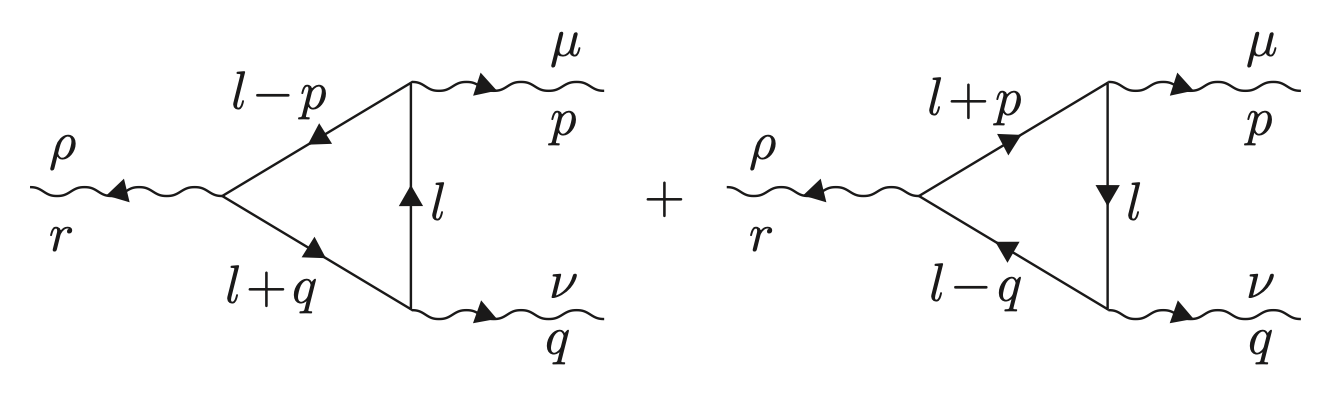
\includegraphics[width=0.5\linewidth,align=c]{pics/AN-Tri-2.png}.
\end{equation}
Note that in the above diagram, all fermion lines are chiral -- they involve only left-handed spinor.
We can evaluate the diagram by replacing all the chiral fermion lines with Dirac fermion lines, plus an additional projector inserted: 
\begin{equation}
	\tr\left[\frac{1-\gamma^5}{2} (\cdots)\right] = \frac{1}{2}\tr\left[(\cdots)\right] - \frac{1}{2}\tr\left[\gamma^5 (\cdots)\right].
\end{equation}
The first term is just an ordinary photon vertex in QED, which is not anomalous.
The second term, however, is exactly the triangle diagram producing the chiral anomaly.
Here the axial current is coupled to the gauge field, the result, we know from the previous calculation that
\begin{equation}
	(p_\mu + q_\nu + r_\rho)\mathcal M^{\mu\nu\rho} 
	= -\frac{ie^3}{4\pi^2}\varepsilon^{\mu\nu\rho\sigma} p_\rho q_\sigma
	= -\frac{ie^3}{4\pi^2}\varepsilon^{\mu\nu\rho\sigma} q_\rho r_\sigma
	= -\frac{ie^3}{4\pi^2}\varepsilon^{\mu\nu\rho\sigma} r_\rho p_\sigma.
\end{equation}
We conclude from this the QED with charged single-handed Weyl fermion is not consistent.
Moreover, if we consider a chiral theory, where the left- and right- handed spinors have different charges.
The triangle diagram is the sum of all Weyl spinors.
The anomalous-free condition is thus
\begin{equation}
	\sum_{i=1}^{N_L} q_{Li}^3 = \sum_{j=1}^{N_R} q_{Rj}^3.
\end{equation}
In standard model, the $\mathrm{U}(1)_{\mathrm{Y}}^3$ anomaly cancels out.
To see this, consider the first-generation fermions:
\begin{equation}
\begin{tabular}{c|cc|cccc}
	\hline
	   & $Q$ & $L$  & $u_R$ & $d_R$ & $e_R$ & $\nu_{eR}$ \\ \hline
	6Y & $1$ & $-3$ & $4$   & $-2$  & $-6$  & $0$        \\
	\hline
\end{tabular}
\end{equation}
Here we write the hypercharge in the unit of $1/6$, the difference between left and right-hand spinor is
\begin{equation}
	\sum_{i=1}^{N_L} (6Y_{Li})^3 - \sum_{j=1}^{N_R} (6Y_{Rj})^3 
	= \left[1^3 \times 6 + (-3)^3 \times 2 \right] -
	\left[4^3 \times 3 + (-2)^3 \times 3 + (-6)^3 \right] 
	= 0.
\end{equation}
We remark that the quark sector or lepton sector alone will lead to $\mathrm{U}(1)_{\mathrm{Y}}^3$ anomaly.
It is the combination of them that makes the gauge theory consistent.




\subsection{Nonabelian Gauge}

We are now considering the nonabelian gauge anomaly.
As a convention, we absorb the coupling constant into the Lie algebra $A^a T^a_R$.
The perturbative anomaly still comes from the triangle diagram.
We have seen that the outcome 3-point vertex is symmetric under changing the external legs.
It means, when coupled to the gauge field $A = A^a T^a$, there will be an additional factor
\begin{equation}
	\tr\left[T_R^a \{T_R^b, T_R^c\}\right] = d^{abc}(R) = A(R) d^{abc}(\text{fund}).
\end{equation}
We see that the symmetric coefficients $d^{abc}$ is related to the anomaly of the nonabelian gauge anomaly.
Following the same logic, the anomaly cancellation condition is
\begin{equation}
	\sum_{i=1}^{N_L} d^{abc}(R_{Li}) = \sum_{j=1}^{N_R} d^{abc}(R_{Rj}).
\end{equation}
Note that for the abelian case, the generator is $qI$, and the symmetric coefficient is $d^{111} = q^3$, which leads to the same condition.
One important fact about the coefficients $d^{abc}$ is that it vanishes for real or pseudoreal representations.
To see this, we first note that the generators are hermitian.
The generators of the conjugate representation is
\begin{equation}
	\bar T^a = - (T^{a})^* = - (T^{a})^T.
\end{equation}
A real or pseudoreal representation means $T^a \sim \bar T^a$, which leads to
\begin{equation}
\begin{aligned}
	d^{abc}(R) 
	&= \tr\left[T^a_R \left\{T^b_R, T^c_R \right\} \right] 
	= \tr\left[\bar T_R^a \left\{\bar T_R^b, \bar T_R^c \right\} \right] \\
	&= -\tr\left[(T_R^a)^T \left\{(T_R^b)^T,(T_R^c)^T \right\} \right] \\
	&= -\tr\left[T_R^a \left\{T_R^b,T_R^c \right\} \right] = 0.
\end{aligned}
\end{equation}



\end{document}


